\begin{enumerate}[label=\thesection.\arabic*,ref=\thesection.\theenumi]
\item Find the sum of the vectors $\vec{a}=\hat{i}-2\hat{j}+\hat{k}$, $\vec{b}=-2\hat{i}+4\hat{j}+5\hat{k}$ and $\vec{c}=\hat{i}-6\hat{j}-7\hat{k}$.
\item 

	In triangle ABC (Fig 10.18), which of the following is not true:
 \begin{enumerate}
         \item $\overrightarrow{AB}+\overrightarrow{BC}+\overrightarrow{CA}$=$\vec{0}$
         \item $\overrightarrow{AB}+\overrightarrow{BC}-\overrightarrow{CA}$=$\vec{0}$
         \item $\overrightarrow{AB}+\overrightarrow{BC}-\overrightarrow{CA}$=$\vec{0}$
         \item $\overrightarrow{AB}-\overrightarrow{BC}+\overrightarrow{CA}$=$\vec{0}$
\end{enumerate}
\begin{figure}[h]
\centering
\includegraphics[width = \columnwidth]{./chapters/12/10/2/18/figs/triangle.png}
\caption{}
	\label{fig:chapters/12/10/2/18/}
\end{figure}
\solution
		\documentclass{article}
\usepackage{amsmath}
\usepackage{xcolor}
\usepackage{gensymb}
\usepackage{ragged2e}
\usepackage{graphicx}
\usepackage{gensymb}
\usepackage{mathtools}
\newcommand{\mydet}[1]{\ensuremath{\begin{vmatrix}#1\end{vmatrix}}}
\providecommand{\brak}[1]{\ensuremath{\left(#1\right)}}
\providecommand{\norm}[1]{\left\lVert#1\right\rVert}
\newcommand{\solution}{\noindent \textbf{Solution: }}
\newcommand{\myvec}[1]{\ensuremath{\begin{pmatrix}#1\end{pmatrix}}}
\let\vec\mathbf
\begin{document}
\begin{center}
        \textbf\large{CHAPTER-7 \\ TRIANGLES}
\end{center}
\section{Exercise 7.1}
Q2. $ABCD$ is a quadrilateral in which $AD = BC$ and $\angle{DAB} = \angle{CBA}$ as shown in figure \ref{fig:Fig}. Prove that
\begin{enumerate}
\item $\triangle{ABD} \cong \triangle{BAC}$
  \item $BD = AC$
  \item $\angle{ABD} = \angle{BAC}$
\end{enumerate}
\textbf{Construction}\\
\begin{figure}[h!]
	\begin{center}
		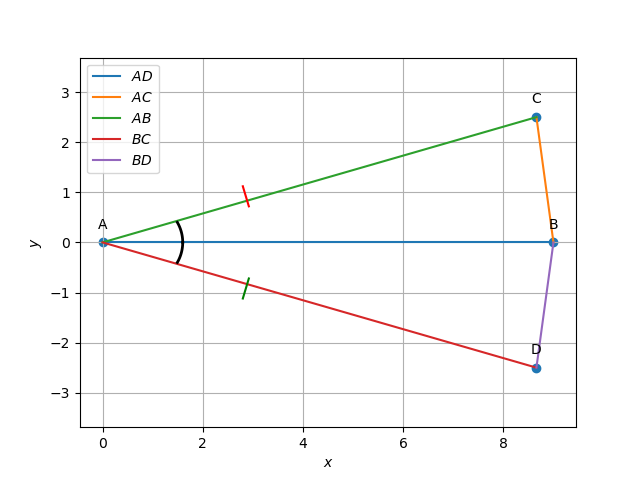
\includegraphics[width=\columnwidth]{figs/graph.png}
	\end{center}
	\caption{Quadrilateral ABCD}
	\label{fig:Fig}
\end{figure}
The input parameters for construction are shown in \ref{tab:Table1}:\\
\begin{table}[h!]
    \centering
    \begin{tabular}{|p{3cm}|p{3cm}|p{3cm}|}
\hline                                        
	\textbf{Symbol} & \textbf{Values} & \textbf{Description} \\                                          
\hline                                 
	a & 3 & $AD=BC$ \\        
\hline                                    
	b & 8 & $AB$ \\    
\hline                      
	$\vec{e}_1$ & $\myvec{1\\0}$ & basis vector \\
\hline
\end{tabular}

    \caption{Parameters}
    \label{tab:Table1}
\end{table}
\pagebreak
\begin{align}
\vec{A} =& \myvec{0\\0},\vec{B} = \myvec{a\\0},\vec{C} = \myvec{c\cos\theta\\c\sin\theta},\vec{D} = \myvec{-c\cos\theta\\c\sin\theta}
\end{align}
\solution
\begin{align}
	\vec{A}-\vec{D} = \vec{B}-\vec{C}\\
  \angle{DAB} = \angle{CBA}
\end{align}
\textbf{To Prove:}
  \begin{align}
	  \triangle{ACB} &\cong \triangle{ADB}\\
	  BD &= AC\\
	  \angle{ABD} &= \angle{BAC}
  \end{align}
\textbf{Proof:}\\
In $\triangle{ABD}$ and $\triangle{BAC}$\\
Let  equation of $AB$ be $y = 0$, which can be written as:
\begin{align}
	\vec{n}^{\top}\vec{x} = 0,\\
\end{align}
\begin{align}
\vec{x} =& \myvec{x\\y},\vec{n} = \myvec{1\\0}\\
\end{align}
  From the above assumptions, we get the coordinates of $C$ and $D$ as
  \begin{align}
\vec{C} =& \myvec{4.3\\-2.5},\vec{D} = \myvec{-4.3\\-2.5}\\
  \end{align}
    Finding the angles(according to assumptions):
    \begin{align}
\text{Let }\theta_1=&\angle ADB\\
\vec{m_1}=&\vec{D}-\vec{A}=\myvec{-4.7\\-2.5}, \vec{m_2}=\vec{D}-\vec{B}=\myvec{-13.7\\-2.5}\\
\theta_1=&\cos^{-1}\frac{\vec{m_1}^\top\vec{m_2}}{\norm{\vec{m_1}}\norm{\vec{m_2}}}\\
\implies\theta_1=&\cos^{-1}\frac{\myvec{-4.7&-2.5}\myvec{-13.7\\-2.5}}{(9.2)(15.8)}=61\degree 
\label{eq:1}\\
\text{ Let }\theta_2=\angle ACB\\
\vec{n_1}=&\vec{C}-\vec{A}=\myvec{4.7\\-2.5}, \vec{n_2}=\vec{C}-\vec{B}=\myvec{13.7\\-2.5}\\
\theta_2 =& \cos^{-1}\frac{\vec{n_1}^\top\vec{n_2}}{\norm{\vec{n_1}}\norm{\vec{n_2}}}\\
\implies\theta_2=&\cos^{-1}\frac{\myvec{4.7&-2.5}\myvec{13.7\\-2.5}}{(9.2)(15.8)}=61\degree 
\label{eq:2}
\end{align}
from $\eqref{eq:1}$ and $\eqref{eq:2}$
\begin{center}
$\angle$ ABD = $\angle$ CAB \text{ (Sum of the angles in a triangle is 180\degree) }
\end{center}
Since all the angles and sides of triangles $CAB$ and $CAD$ are equal , from the definition of congruency both the triangles are said to be congruent to each other.
\begin{align}
    \triangle{ACB} & \cong \triangle{ADB}\\
    BD &= AC\\
    \angle{ABD} &= \angle{BAC}
\end{align}
\end{document}


\item If $\vec{a}$ and $\vec{b}$ are two collinear vectors, then which of the following are incorrect:
\begin{enumerate}
    \item $\vec{b}=\lambda\vec{a},$
 for some scalar $\lambda$
    \item $\vec{a}=\pm\vec{b}$
    \item the respective components of $\vec{a}$ and $\vec{b}$ are not proportiona
    \item both the vectors $\vec{a}$ and $\vec{b}$ have same direction, but different magnitudes.
\end{enumerate}
	\item If a line makes angles $90\degree,135\degree,45\degree$ with x,y and z-axis respectivly. Find its direction cosines.
		\\
		\solution
		\input{chapters/12/11/1/1/vec.tex}
\item A girl walks 4 km towards west, then she walks 3 km in a direction 30$^{\circ}$ east of north and stops. Determine the girl's displacement from her initial point of departure.\\
	\solution
		\input{chapters/12/10/5/3/vec.tex}
\item If $\vec{a}=\hat{i}+\hat{j}+\hat{k}$,$\vec{b}=2\hat{i}-\hat{j}+3\hat{k}$ and $\vec{c}=\hat{i}-2\hat{j}+\hat{k}$, find a unit vector parallel to the vector $2\vec{a}-\vec{b}+3\vec{c}$.\\
	\solution
		\input{chapters/12/10/5/7/norm.tex}
\item The two opposite vertices of a square are $(–1, 2)$  and $ (3, 2)$. Find the coordinates of the other two vertices.
\\
	\input{chapters/10/7/4/4/affine.tex}
\item The base of an equilateral triangle with side $2a$ lies along the y-axis such that the mid-point of the base is at the origin. Find vertices of the triangle.
\label{chapters/11/10/1/2}
\input{chapters/11/10/1/2/matrix.tex}
\item Without using distance formula, show that points (– 2, – 1), (4, 0), (3, 3) and (–3, 2) are the vertices of a parallelogram.
\label{chapters/11/10/1/9}
\documentclass{article}
\usepackage{amsmath}
\usepackage{xcolor}
\usepackage{gensymb}
\usepackage{ragged2e}
\usepackage{graphicx}
\usepackage{gensymb}
\usepackage{mathtools}
\newcommand{\mydet}[1]{\ensuremath{\begin{vmatrix}#1\end{vmatrix}}}
\providecommand{\brak}[1]{\ensuremath{\left(#1\right)}}
\providecommand{\norm}[1]{\left\lVert#1\right\rVert}
\newcommand{\solution}{\noindent \textbf{Solution: }}
\newcommand{\myvec}[1]{\ensuremath{\begin{pmatrix}#1\end{pmatrix}}}
\let\vec\mathbf
\begin{document}
\begin{center}
        \textbf\large{CHAPTER-7 \\ TRIANGLES}
\end{center}
\section{Exercise 7.1}
Q2. $ABCD$ is a quadrilateral in which $AD = BC$ and $\angle{DAB} = \angle{CBA}$ as shown in figure \ref{fig:Fig}. Prove that
\begin{enumerate}
\item $\triangle{ABD} \cong \triangle{BAC}$
  \item $BD = AC$
  \item $\angle{ABD} = \angle{BAC}$
\end{enumerate}
\textbf{Construction}\\
\begin{figure}[h!]
	\begin{center}
		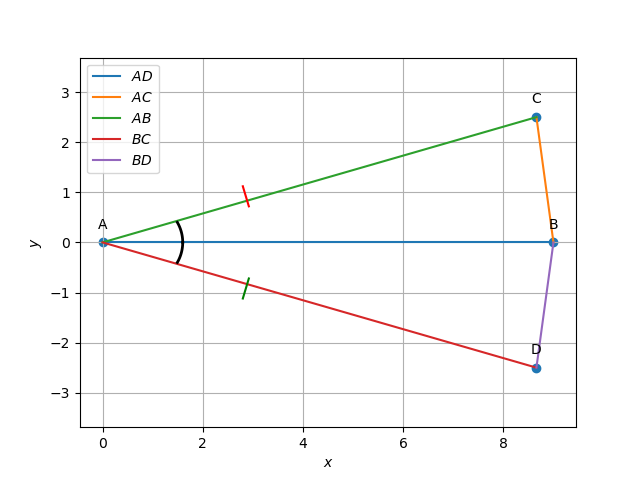
\includegraphics[width=\columnwidth]{figs/graph.png}
	\end{center}
	\caption{Quadrilateral ABCD}
	\label{fig:Fig}
\end{figure}
The input parameters for construction are shown in \ref{tab:Table1}:\\
\begin{table}[h!]
    \centering
    \begin{tabular}{|p{3cm}|p{3cm}|p{3cm}|}
\hline                                        
	\textbf{Symbol} & \textbf{Values} & \textbf{Description} \\                                          
\hline                                 
	a & 3 & $AD=BC$ \\        
\hline                                    
	b & 8 & $AB$ \\    
\hline                      
	$\vec{e}_1$ & $\myvec{1\\0}$ & basis vector \\
\hline
\end{tabular}

    \caption{Parameters}
    \label{tab:Table1}
\end{table}
\pagebreak
\begin{align}
\vec{A} =& \myvec{0\\0},\vec{B} = \myvec{a\\0},\vec{C} = \myvec{c\cos\theta\\c\sin\theta},\vec{D} = \myvec{-c\cos\theta\\c\sin\theta}
\end{align}
\solution
\begin{align}
	\vec{A}-\vec{D} = \vec{B}-\vec{C}\\
  \angle{DAB} = \angle{CBA}
\end{align}
\textbf{To Prove:}
  \begin{align}
	  \triangle{ACB} &\cong \triangle{ADB}\\
	  BD &= AC\\
	  \angle{ABD} &= \angle{BAC}
  \end{align}
\textbf{Proof:}\\
In $\triangle{ABD}$ and $\triangle{BAC}$\\
Let  equation of $AB$ be $y = 0$, which can be written as:
\begin{align}
	\vec{n}^{\top}\vec{x} = 0,\\
\end{align}
\begin{align}
\vec{x} =& \myvec{x\\y},\vec{n} = \myvec{1\\0}\\
\end{align}
  From the above assumptions, we get the coordinates of $C$ and $D$ as
  \begin{align}
\vec{C} =& \myvec{4.3\\-2.5},\vec{D} = \myvec{-4.3\\-2.5}\\
  \end{align}
    Finding the angles(according to assumptions):
    \begin{align}
\text{Let }\theta_1=&\angle ADB\\
\vec{m_1}=&\vec{D}-\vec{A}=\myvec{-4.7\\-2.5}, \vec{m_2}=\vec{D}-\vec{B}=\myvec{-13.7\\-2.5}\\
\theta_1=&\cos^{-1}\frac{\vec{m_1}^\top\vec{m_2}}{\norm{\vec{m_1}}\norm{\vec{m_2}}}\\
\implies\theta_1=&\cos^{-1}\frac{\myvec{-4.7&-2.5}\myvec{-13.7\\-2.5}}{(9.2)(15.8)}=61\degree 
\label{eq:1}\\
\text{ Let }\theta_2=\angle ACB\\
\vec{n_1}=&\vec{C}-\vec{A}=\myvec{4.7\\-2.5}, \vec{n_2}=\vec{C}-\vec{B}=\myvec{13.7\\-2.5}\\
\theta_2 =& \cos^{-1}\frac{\vec{n_1}^\top\vec{n_2}}{\norm{\vec{n_1}}\norm{\vec{n_2}}}\\
\implies\theta_2=&\cos^{-1}\frac{\myvec{4.7&-2.5}\myvec{13.7\\-2.5}}{(9.2)(15.8)}=61\degree 
\label{eq:2}
\end{align}
from $\eqref{eq:1}$ and $\eqref{eq:2}$
\begin{center}
$\angle$ ABD = $\angle$ CAB \text{ (Sum of the angles in a triangle is 180\degree) }
\end{center}
Since all the angles and sides of triangles $CAB$ and $CAD$ are equal , from the definition of congruency both the triangles are said to be congruent to each other.
\begin{align}
    \triangle{ACB} & \cong \triangle{ADB}\\
    BD &= AC\\
    \angle{ABD} &= \angle{BAC}
\end{align}
\end{document}

\item A line passes through $(x_1,y_1)$ and $(h,k)$. If slope of the line is m show that $(k-y_1)=m(h-x_1)$.
\label{chapters/11/10/1/12}
\input{chapters/11/10/1/12/matrix.tex}
\item Consider the following population and year graph, Find the slope of the line AB and using it, find what will be the population in the year 2010?
\\
\begin{figure}[ht]
\centering
\includegraphics[width = \columnwidth]{chapters/11/10/1/14/figs/fig.png}
\caption{}
\label{fig:chapters/11/10/1/14/1}
\end{figure}
\solution
%\documentclass[12pt]{article}
%\usepackage[cmex10]{amsmath}
%\usepackage{amsthm}
%\usepackage{mathrsfs}
%\usepackage{txfonts}
%\usepackage{stfloats}
%\usepackage{bm}
%\usepackage{cite}
%\usepackage{cases}
%\usepackage{subfig}
%\usepackage{longtable}
%\usepackage{multirow}
%\usepackage{enumitem}
%\usepackage{mathtools}
%\usepackage{steinmetz}
%\usepackage{tikz}
%\usepackage{circuitikz}
%\usepackage{verbatim}
%\usepackage{tfrupee}
%\usepackage[breaklinks=true]{hyperref}
%\usepackage{tkz-euclide} % loads  TikZ and tkz-base
%\providecommand{\brak}[1]{\ensuremath{\left(#1\right)}}
%\usepackage{atbegshi}
%\AtBeginDocument{\AtBeginShipoutNext{\AtBeginShipoutDiscard}}
%\usetikzlibrary{calc,math}
%\usepackage{listings}
%    \usepackage{color}                                            %%
%    \usepackage{array}                                            %%
 %   \usepackage{longtable}                                        %%
  %  \usepackage{calc}                                             %%
   % \usepackage{multirow}                                         %%
    %\usepackage{hhline}                                           %%
    %\usepackage{ifthen}                                           %%
  %optionally (for landscape tables embedded in another document): %%
    %\usepackage{lscape}     
%\usepackage{multicol}
%\usepackage{chngcntr}

%\DeclareMathOperator*{\Res}{Res}
%\renewcommand{\baselinestretch}{2}
%\renewcommand\thesection{\arabic{section}}
%\renewcommand\thesubsection{\thesection.\arabic{subsection}}
%\renewcommand\thesubsubsection{\thesubsection.\arabic{subsubsection}}


% correct bad hyphenation here
%\hyphenation{op-tical net-works semi-conduc-tor}
%\def\inputGnumericTable{}                                 %%

%\lstset{
%language=C,
%frame=single, 
%breaklines=true,
%columns=fullflexible
%}
%\begin{document}
%\newtheorem{theorem}{Theorem}[section]
%\newtheorem{problem}{Problem}
%\newtheorem{proposition}{Proposition}[section]
%\newtheorem{lemma}{Lemma}[section]
%\newtheorem{corollary}[theorem]{Corollary}
%\newtheorem{example}{Example}[section]
%\newtheorem{definition}[problem]{Definition}
%\newcommand{\BEQA}{\begin{eqnarray}}
%\newcommand{\EEQA}{\end{eqnarray}}
%\newcommand{\define}{\stackrel{\triangle}{=}}

%\bibliographystyle{IEEEtran}
%\bibliographystyle{ieeetr}
%\providecommand{\mbf}{\mathbf}
%\providecommand{\pr}[1]{\ensuremath{\Pr\left(#1\right)}}
%\providecommand{\qfunc}[1]{\ensuremath{Q\left(#1\right)}}
%\providecommand{\sbrak}[1]{\ensuremath{{}\left[#1\right]}}
%\providecommand{\lsbrak}[1]{\ensuremath{{}\left[#1\right.}}
%\providecommand{\rsbrak}[1]{\ensuremath{{}\left.#1\right]}}
%\providecommand{\brak}[1]{\ensuremath{\left(#1\right)}}
%\providecommand{\lbrak}[1]{\ensuremath{\left(#1\right.}}
%\providecommand{\rbrak}[1]{\ensuremath{\left.#1\right)}}
%\providecommand{\cbrak}[1]{\ensuremath{\left\{#1\right\}}}
%\providecommand{\lcbrak}[1]{\ensuremath{\left\{#1\right.}}
%\providecommand{\rcbrak}[1]{\ensuremath{\left.#1\right\}}}
%\theoremstyle{remark}
%\newtheorem{rem}{Remark}
%\newcommand{\sgn}{\mathop{\mathrm{sgn}}}
%\providecommand{\res}[1]{\Res\displaylimits_{#1}} 
%\providecommand{\mtx}[1]{\mathbf{#1}}
%\providecommand{\fourier}{\overset{\mathcal{F}}{\rightleftharpoons}}
%\providecommand{\system}{\overset{\mathcal{H}}{\longleftrightarrow}}
	%\newcommand{\solution}[2]{\textbf{Solution:}{#1}}
%\newcommand{\solution}{\noindent \textbf{Solution: }}
%\newcommand{\cosec}{\,\text{cosec}\,}
%\providecommand{\dec}[2]{\ensuremath{\overset{#1}{\underset{#2}{\gtrless}}}}
%\newcommand{\myvec}[1]{\ensuremath{\begin{pmatrix}#1\end{pmatrix}}}
%\newcommand{\mydet}[1]{\ensuremath{\begin{vmatrix}#1\end{vmatrix}}}
%\let\vec\mathbf
%\begin{center}
%\title{\textbf{Straight Lines}}
%\date{\vspace{-5ex}} %Not to print date automatically
%\maketitle
%\end{center}
%\setcounter{page}{1}
%\section*{11$^{th}$ Maths - Chapter 10}
%This is Problem-10 from Exercise 10.4
%\begin{enumerate}
%    \item If three lines whose equations are $y=m_1x+c_1$, $y=m_2x+c_2$ and $y=m_3x+c_3$ are concurrent, then show that $m_1(c_2-c_3)+m_2(c_3-c_1)+m_3(c_1-c_2) = 0.$\\
%    \solution 
    Given lines can be written as \begin{align}
       m_1x-y+c_1=0
    \end{align}
    \begin{align}
        m_2x-y+c_2=0
    \end{align}
    \begin{align}
        m_3x-y+c_3=0
        \label{eq:line3}
    \end{align}
    
    
   The above lines can be written in the form of \begin{align}
        \vec{n}^{\top}\vec{x} = c
    \end{align}
   Therefore,
		\begin{align}
       \myvec{m_1&-1}\vec{x}=c_1
       \label{eq:line5}
   \end{align} 
   \begin{align}
       \myvec{m_2&-1}\vec{x}=c_2
       \label{eq:line6}
   \end{align}
   \begin{align}
       \myvec{m_3&-1}\vec{x}=c_3
       \label{eq:line7}
   \end{align}
   Solving equations \eqref{eq:line5}, \eqref{eq:line6}and \eqref{eq:line7}
		augumented matrix is
 \begin{align}
    \myvec{m_1&-1&c_1\\m_2&-1&c_2\\m_3&-1&c_3}\\
    \xleftrightarrow{R_2 \leftarrow m_1R_2-m_2R_1}
    \myvec{m_1&-1&c_1\\0&m_2-m_1&m_1c_2-m_2c_1\\m_3&-1&c_3}\\
    \xleftrightarrow{R_3 \leftarrow m_1R_3-m_3R_1}
    \myvec{m_1&-1&c_1\\0&m_2-m_1&m_1c_2-m_2c_1\\0&m_3-m_1&m_1c_3-m_3c_1}\\
    \xleftrightarrow{R_3 \leftarrow R_3\frac{m_2-m_1}{m_3-m_1}-R_2}
        \myvec{m_1&-1&c_1\\0&m_2-m_1&m_1c_2-m_2c_1\\0&0&$\brak{m_1c_3-m_3c_1}$$\brak{\frac{m_2-m_1}{m_3-m_1}}$-$\brak{m_1c_2-m_2c_1}$}
\end{align}
Now, for lines to be concurrent, then the third row should be equal to zero. \\

Therefore,
\begin{align}
\brak{m_1c_3-m_3c_1}\brak{\frac{m_2-m_1}{m_3-m_1}}-\brak{m_1c_2-m_2c_1}=0\\
\frac{\brak{m_1c_3-m_3c_1}\brak{m_2-m_1}-\brak{m_1c_2-m_2c_1}\brak{m_3-m_1}}{m_3-m_1}=0\\
\brak{m_1c_3-m_3c_1}\brak{m_2-m_1}-\brak{m_1c_2-m_2c_1}\brak{m_3-m_1}=0\\
m_2c_3-m_1c_3+m_3c_1-m_3c_2+m_1c_2-m_2c_1=0\\
m_1\brak{c_2-c_3}+m_2\brak{c_3-c_1}+m_3\brak{c_1-c_2} = 0
\end{align}
           Hence proved
%\begin{figure}[h]
 %   \centering
  %  \includegraphics[width=\columnwidth]{concurrent-1.png}
   % \caption{Straight Lines}
    %\label{fig:concurrent-1.png}
%\end{figure}
%\end{enumerate}
%\end{document}

\item Find a vector of magnitude 5 units, and parallel to the resultant of the vectors $\vec{a}=2\hat{i}+3\hat{j}-\hat{k}$ and $\vec{b}=\hat{i}-2\hat{j}+\hat{k}$.\\

\item Let $\vec{a}$ and $\vec{b}$ be two unit vectors and $\theta$ is the angle between them. Then $\vec{a}+\vec{b}$ is a unit vector if
		\begin{tasks}(4)
			\task $\theta = \frac{\pi}{4}$
			\task $\theta = \frac{\pi}{3}$
			\task $\theta = \frac{\pi}{2}$
			\task $\theta = \frac{2\pi}{3}$
			\end{tasks}
\solution
\documentclass{article}
\usepackage{amsmath}
\usepackage{setspace}
\usepackage{tasks}
\usepackage{graphicx}
\usepackage{listings}

\newcommand{\solution}{\noindent \textbf{Solution: }}
\newcommand{\norm}[1]{\lVert#1\rVert}
\renewcommand{\vec}[1]{\textbf{#1}}
\begin{document}
\onehalfspacing
\begin{center}
	\section*{\textbf{Class 12}}
	\subsection*{Chapter 10 - Vector Algebra}
\end{center}
The following problem is question 17 from exercise 10.5

\begin{enumerate}
	\item Let $\vec{a}$ and $\vec{b}$ be two unit vectors and $\theta$ is the angle between them. Then $\vec{a}+\vec{b}$ is a unit vector if
		\begin{tasks}(4)
			\task $\theta = \frac{\pi}{4}$
			\task $\theta = \frac{\pi}{3}$
			\task $\theta = \frac{\pi}{2}$
			\task $\theta = \frac{2\pi}{3}$
			\end{tasks}
			
\end{enumerate}
\solution
Given,
\begin{align}
	\norm{\vec{a}}=\norm{\vec{b}}=1\label{eq:1}
	\\
	\norm{\vec{a}+\vec{b}}=1\label{eq:2}
\end{align}
Squaring both sides of \eqref{eq:2}  , we get
\begin{align}
	\norm{\vec{a}+\vec{b}}^2=1^2
\\	
	\implies \norm{\vec{a}}^2 + \norm{\vec{b}}^2 + 2\vec{a}^{\top}\vec{b} = 1\label{eq:3}	
\end{align}
Substituting \eqref{eq:1} in \eqref{eq:3}, we get
\\
\begin{align}
	\implies 1+1+2(\norm{\vec{a}}\norm{\vec{b}}\cos{\theta})=1
	\\
	\implies 2+2(\norm{\vec{a}}\norm{\vec{b}}\cos{\theta})=1
        \\
	\implies 2(\norm{\vec{a}}\norm{\vec{b}}\cos{\theta})=-1
	\\
	\implies (\norm{\vec{a}}\norm{\vec{b}}\cos{\theta})=\frac{-1}{2}\label{eq:4}
\end{align}
Subtituting \eqref{eq:1} in \eqref{eq:4}, we get
\begin{align}
	\implies \cos{\theta}=\frac{-1}{2}
	\\
	\implies \theta=\frac{2\pi}{3}
\end{align}
\begin{figure}[!h]
	\begin{center}
	\includegraphics[width=\columnwidth]{codes/Python/figs/fig.png}
	\end{center}
	\caption{$\vec{OA}$ and $\vec{CO}$ is $\vec{a}$ and $\vec{OB}$ is $\vec{b}$ and $\vec{CB}$ is $\vec{a+b}$}
	\label{fig:12/10/5/17}
\end{figure}
\end{document}


\end{enumerate}
